\nonstopmode

\documentclass[twoside,letterpaper]{article}
% \usepackage{a4}
\usepackage[latin1]{inputenc}
\usepackage[T1]{fontenc}
\usepackage{latexsym}
\usepackage{makeidx}
\usepackage{verbatim}

\usepackage{fancyhdr}

\usepackage{ifpdf}
\newif\ifpdf
\ifx\pdfoutput\undefined
\else
  \ifx\pdfoutput\relax
  \else
    \ifcase\pdfoutput
    \else
      \pdftrue
    \fi
  \fi
\fi
\ifpdf
  \usepackage[pdftex,colorlinks=true,bookmarksopen, pdfstartview=FitH,
              linkcolor=blue, citecolor=blue, urlcolor=blue]{hyperref}
  \usepackage[pdftex]{graphicx}
  \pdfcompresslevel=9
\else
  \usepackage[dvips]{graphicx}
\fi



\usepackage{ae}
\usepackage{aecompl}


% HORIZONTAL MARGINS
% Left margin, odd pages: 1.25 inch (0.25 + 1)
\setlength{\oddsidemargin}{0.25in}
% Left margin, even pages: 1.25 inch (0 + 1)
\setlength{\evensidemargin}{0.25in}
% Text width 6 inch (so other margin is 1.25 inch).
\setlength{\textwidth}{6in}
% ----------------
% VERTICAL MARGINS
% Top margin 0.5 inch (-0.5 + 1)
\setlength{\topmargin}{-0.5in}
% Head height 0.25 inch (where page headers go)
\setlength{\headheight}{0.25in}
% Head separation 0.25 inch (between header and top line of text)
\setlength{\headsep}{0.25in}
% Text height 9 inch (so bottom margin 1 in)
\setlength{\textheight}{9in}
% ----------------
% PARAGRAPH INDENTATION
\setlength{\parindent}{0in}
% SPACE BETWEEN PARAGRAPHS
\setlength{\parskip}{\medskipamount}
% ----------------
% STRUTS
% HORIZONTAL STRUT.  One argument (width).
\newcommand{\hstrut}[1]{\hspace*{#1}}
% VERTICAL STRUT. Two arguments (offset from baseline, height).
\newcommand{\vstrut}[2]{\rule[#1]{0in}{#2}}
% ----------------
% HORIZONTAL LINE ACROSS PAGE:
\newcommand{\hdivider}{\noindent\mbox{}\hrulefill\mbox{}} 
% ----------------
% EMPTY BOXES OF VARIOUS WIDTHS, FOR INDENTATION
\newcommand{\hm}{\hspace*{1em}}
\newcommand{\hmm}{\hspace*{2em}}
\newcommand{\hmmm}{\hspace*{3em}}
\newcommand{\hmmmm}{\hspace*{4em}}
% ----------------

\newcommand{\te}[1]{\texttt{#1}}

\newenvironment{libverbatim}
  {\vspace*{-1.0em}
   \verbatim}
  {\endverbatim
  }

% \title{
% {\BS}$^{\rm{TM}}$ {\SV} \\
% Version {\BSVVersion} \\
% Reference Guide \\
% \vspace*{1in}
% {\large\bf Please do not circulate without permission from Bluespec, Inc.} \\
% \vspace*{1in}
% \mbox{}
% }

%\input{../common_dates.tex}

\begin{document}


 \section{AHB}
% \label{sec-AHB}
% \index{AHB}
% \index[bsvsource]{AHB}
% \index[bsvsource]{AHBBus}
% \index[bsvsource]{AHBDefines}
% \index[bsvsource]{AHBMaster}
% \index[bsvsource]{AHBMonitor}
% \index[bsvsource]{AHBPC}
% \index[bsvsource]{AHBSlave}

{\bf Packages}
% \index{AHB (package)}

\begin{verbatim}
import AHB :: * ;
\end{verbatim}







{\bf Description}

The AHB library includes interface, transactor,  module and
function definitions to
implement the AHB protocol with Bluespec SystemVerilog.  The BSV AHB
library  groups the AHB data and protocols
into  reusable, parameterized
interfaces, which interact with TLM interfaces.  An AHB bus is
implemented  using AHB transactors  -
interfaces  which connect TLM interfaces on one side with
AHB interfaces on the other side.  


The AHB library supports the following AHB Bus protocol features:
\begin{itemize}
\item Basic and Burst Transfers
\item Locked Transfers
\end{itemize}

The AHB library does not support the following  AHB Bus protocol features:
\begin{itemize}
\item Early Burst Termination
\item Split Transfers
\item Retry Transfers
\end{itemize}

\begin{figure}[ht]
\begin{center}
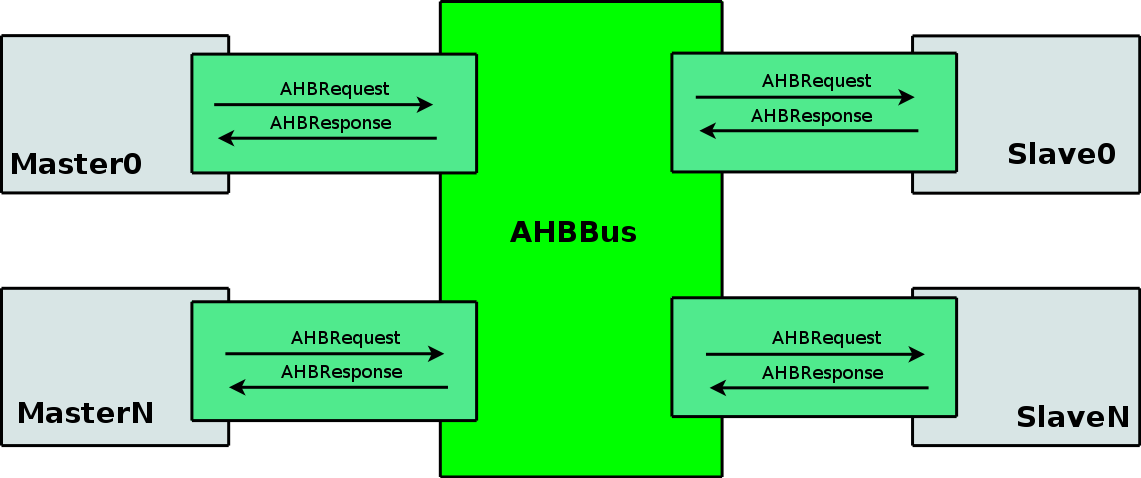
\includegraphics[height = 2 in]{AHBex2}
\caption{AHB Bus Example}
\label{AHBbus}
\end{center}
\end{figure}


{\bf Data Structures}
% \index{AHBData@\te{AHBData} (data type)}
% \index{AHBAddr@\te{AHBAddr} (data type)}
% \index{AHBWrite@\te{AHBWrite} (data type)}
% \index{AHBResponse@\te{AHBResponse} (data type)}
% \index{AHBTransfer@\te{AHBTransfer} (data type)}
% \index{AHBBurst@\te{AHBBurst} (data type)}
% \index{AHBProt@\te{AHBProt} (data type)}

Inside the transactor modules, the AHB data is organized into the
following data structures: the address and control information is
defined by \te{AHBCtrl}, the write data is defined by \te{AHBData}.
These two structures are bundled into an \te{AHBRequest}. Finally, 
the response data is defined by \te{AHBResponse}.

\paragraph{\bf AHBRequest}
An AHB request is defined by the \te{AHBRequest} structure as
described below.

\begin{center}
\begin{tabular}{|p{1 in}|p{1.8in}|p{3.2 in}|}
\hline
\multicolumn{3}{|c|}{AHBRequest} \\
\hline
\multicolumn{1}{|c|}{Member}&\multicolumn{1}{|c|}{DataType}&\multicolumn{1}{|c|}{Valid Values} \\
\hline
\hline
cntrl&\te{AHBCtrl\#(`TLM\_PRM)}&see above\\
\hline
data&\te{AHBData\#(`TLM\_PRM)}&\te{Bit\#(data\_size)}\\
\hline
\end{tabular}
\end{center}


\begin{verbatim}
typedef struct {
                AHBCtrl#(`TLM_PRM)    ctrl;
                AHBData#(`TLM_PRM)    data;
               } AHBRequest#(`TLM_PRM_DCL) `dv;

\end{verbatim}

\paragraph{\bf AHBCtrl} The control fields in an \te{AHBRequest} are
                described by the \te{AHBCtrl} structure, the components
                of which are defined in the following table.


\begin{center}
\begin{tabular}{|p{1 in}|p{1.8in}|p{3.2 in}|}
\hline
\multicolumn{3}{|c|}{AHBCtrl} \\
\hline
\multicolumn{1}{|c|}{Member}&\multicolumn{1}{|c|}{DataType}&\multicolumn{1}{|c|}{Valid Values} \\
\hline
\hline
command&\te{AHBWrite}&READ, WRITE\\
\hline
size&\te{AHBSize}&BITS8, BITS16, BITS32, BITS64, BITS128, BITS256,
BITS512, BITS1024\\
\hline
burst&\te{AHBBurst}&SINGLE, INCR, WRAP4, INCR4, WRAP8, INCR8, WRAP16,
INCR16\\
\hline
transfer&\te{AHBTransfer}&IDLE, BUSY, NONSEQ, SEQ\\
\hline
prot&\te{AHBProt}&\te{Bit\#(4)}\\
\hline
addr&\te{AHBAddr\#(`TLM\_PRM)}&\te{Bit\#(addr\_size)}\\
\hline
\end{tabular}
\end{center}

\begin{verbatim}
typedef struct {
                AHBWrite             command;
                AHBSize              size;
                AHBBurst             burst;   
                AHBTransfer          transfer;
                AHBProt              prot;   
                AHBAddr#(`TLM_TYPES) addr;
               } AHBCtrl#(`TLM_PRM_DCL) `dv;

\end{verbatim}



\paragraph{\bf AHBResponse} An \te{AHBResponse} consists of a status
                fields and data (when responding to a read request). 
                The components of the structure are described in the following table.


\begin{center}
\begin{tabular}{|p{1 in}|p{1.8in}|p{3.2 in}|}
\hline
\multicolumn{3}{|c|}{AHBResponse} \\
\hline
\multicolumn{1}{|c|}{Member}&\multicolumn{1}{|c|}{DataType}&\multicolumn{1}{|c|}{Valid Values} \\
\hline
\hline
status&\te{AHBResp}&OKAY, ERROR, RETRY, SPLIT\\
\hline
data&\te{AHBData}&\te{Bit\#(data\_size)}\\
\hline
command&\te{Maybe\#(AHBWrite)}&READ, WRITE\\
\hline
\end{tabular}
\end{center}

\begin{verbatim}
typedef struct {
                AHBResp              status;
                AHBData#(`TLM_PRM) data;
                Maybe#(AHBWrite)     command;
               } AHBResponse#(`TLM_PRM_DCL) `dv;
\end{verbatim}

{\bf Bus Interfaces}

The two basic bus interfaces included in the AHB library are the
\te{AHBMaster} interface and the \te{AHBSlave} interface.

% \begin{figure}[ht]
% \begin{center}
% \includegraphics[height = 1.2 in]{AHBinterfaces}
% \caption{AHB Bus Interfaces}
% \label{AHBSlave}
% \end{center}
% \end{figure}

\paragraph{\bf AHBMaster} The \te{AHBMaster} interface issues AHB requests 
and receives AHB responses. 

\begin{figure}[ht]
\begin{center}
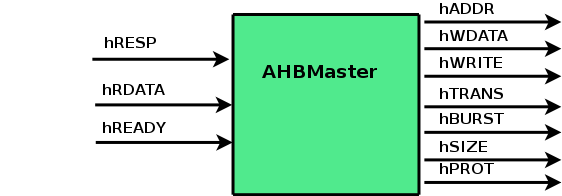
\includegraphics[height = 1 in]{AHBMasterIFC}
\caption{AHB Master Interface}
\label{AHBMaster}
\end{center}
\end{figure}


\begin{verbatim}
(* always_ready, always_enabled *)
interface AHBMaster#(`TLM_PRM_DCL);
   // Outputs
   (* result = "HADDR" *)
   method AHBAddr#(`TLM_PRM)  hADDR;
   (* result = "HWDATA" *)
   method AHBData#(`TLM_PRM)  hWDATA;
   (* result = "HWRITE" *)
   method AHBWrite              hWRITE;
   (* result = "HTRANS" *)
   method AHBTransfer           hTRANS;
   (* result = "HBURST" *)
   method AHBBurst              hBURST;
   (* result = "HSIZE" *)
   method AHBSize               hSIZE;
   (* result = "HPROT" *)
   method AHBProt               hPROT;
   // Inputs
   (* prefix = "", result = "unused0" *)
   method Action      hRDATA((* port = "HRDATA" *) AHBData#(`TLM_PRM) data);
   (* prefix = "", result = "unused1" *)
   method Action      hREADY((* port = "HREADY" *) Bool value);
   (* prefix = "", result = "unused2" *)
   method Action      hRESP((* port = "HRESP" *) AHBResp response);
endinterface
\end{verbatim}

\paragraph{\bf AHBSlave} The \te{AHBSlave} interface receives AHB requests 
and returns AHB responses.

\begin{figure}[ht]
\begin{center}
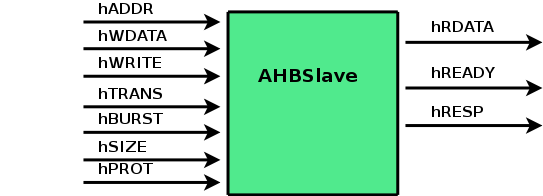
\includegraphics[height = 1 in]{AHBSlaveFC}
\caption{AHB Slave Interface}
\label{AHBSlave}
\end{center}
\end{figure}

\begin{verbatim}
(* always_ready, always_enabled *)
interface AHBSlave#(`TLM_PRM_DCL);
    // Inputs
   (* prefix = "", result = "unused0" *)
   method Action      hADDR((* port = "HADDR" *)    AHBAddr#(`TLM_PRM) addr);
   (* prefix = "", result = "unused1" *)
   method Action      hWDATA((* port = "HWDATA" *)  AHBData#(`TLM_PRM) data);
   (* prefix = "", result = "unused2" *)
   method Action      hWRITE((* port = "HWRITE" *)  AHBWrite    value);
   (* prefix = "", result = "unused3" *)
   method Action      hTRANS((* port = "HTRANS" *)  AHBTransfer value);
   (* prefix = "", result = "unused4" *)
   method Action      hBURST((* port = "HBURST" *)  AHBBurst    value);
   (* prefix = "", result = "unused5" *)
   method Action      hSIZE((* port = "HSIZE" *)    AHBSize     value);
   (* prefix = "", result = "unused6" *)
   method Action      hPROT((* port = "HPROT" *)    AHBProt     value);
   
   // Outputs
   (* result = "HRDATA" *)
   method AHBData#(`TLM_PRM) hRDATA;
   (* result = "HREADY" *)
   method Bool               hREADY;
   (* result = "HRESP" *)
   method AHBResp            hRESP;
endinterface
\end{verbatim}

The \te{AHBMaster} and \te{AHBSlave} interfaces are connectable.

\begin{verbatim}
instance Connectable#(AHBMaster#(`TLM_PRM), AHBSlave#(`TLM_PRM));
\end{verbatim}

%% \begin{verbatim}
%% instance Connectable#(AHBMaster#(`TLM_PRM), AHBSlave#(`TLM_PRM));
%%    module mkConnection#(AHBMaster#(`TLM_PRM) master, 
%%                         AHBSlave#(`TLM_PRM) slave )(Empty);
%% \end{verbatim}



{\bf Fabric Interfaces}

When used in the context of a bus or switch, AHB Master and Slave
modules must communicate with the arbiter and with address decoding
logic. Two additional interfaces are provided to support this
communication.

\paragraph{\bf AHBMasterArbiter} The \te{AHBMasterArbiter} interface 
connects the master module with the bus arbiter.  Through this
interface, the master can request control of the bus and determine
when control has been granted.

\begin{verbatim}
(* always_ready, always_enabled *)
interface AHBMasterArbiter;
   (* result = "HBUSREQ" *)
   method Bool        hBUSREQ;
   (* result = "HLOCK" *)
   method Bool        hLOCK;
   (* prefix = "" *)
   method Action      hGRANT((* port = "HGRANT" *) Bool value);
endinterface
\end{verbatim}


\paragraph{\bf AHBMasterArbiterDual}

\begin{verbatim}
(* always_ready, always_enabled *)
interface AHBMasterArbiterDual;
   (* prefix = "", result = "unused7" *)
   method Action      hBUSREQ((* port = "HBUSREQ" *) Bool value);
   (* prefix = "", result = "unused8" *)
   method Action      hLOCK((* port = "HLOCK" *)     Bool value);
   (* result = "HGRANT" *)
   method Bool hGRANT;
endinterface
\end{verbatim}

\paragraph{\bf AHBSlaveSelector} The \te{AHBSlaveSelector} interface 
provides an \te{addrMatch} method which given an AHB address returns
an Boolean value indicating whether the given address maps to the
associated slave. By polling this method for each slave on the bus,
the decoding logic can determine the appropriate destination for each
bus transaction. The \te{AHBSlaveSelector} interface also provides a
\te{select} method by which the decoding logic can indicate which 
slave is the selected destination.

\begin{verbatim}
interface AHBSlaveSelector#(`TLM_PRM_DCL);
   method Bool   addrMatch(AHBAddr#(`TLM_PRM) value);
   (* prefix = "" *)
   method Action select((* port = "HSEL" *) Bool value);
endinterface
\end{verbatim}

\paragraph{\bf AHBFabricMaster} The \te{AHBFabricMaster} interface 
bundles two subinterfaces, an \te{AHBMaster} interface and an
\te{AHBMasterArbiter} interface.  It is this interface that is 
provided as an argument when constructing an AHB bus and as the bus
side interface of an AHB master transactor module.

\begin{verbatim}
interface AHBFabricMaster#(`TLM_PRM_DCL);
   (* prefix = "" *)
   interface AHBMaster#(`TLM_PRM)  bus;
   (* prefix = "" *)
   interface AHBMasterArbiter        arbiter;
endinterface
\end{verbatim}

\paragraph{\bf AHBFabricSlave} The \te{AHBFabricSlave} interface 
bundles two subinterfaces, an \te{AHBSlave} interface and an
\te{AHBSlaveSelector} interface.  It is this interface that is 
provided as an argument when constructing an AHB bus and as the bus
side interface of an AHB slave transactor module

\begin{verbatim}
interface AHBFabricSlave#(`TLM_PRM_DCL);
   (* prefix = "" *)
   interface AHBSlave#(`TLM_PRM)         bus;
   (* prefix = "" *)
   interface AHBSlaveSelector#(`TLM_PRM) selector;
endinterface
\end{verbatim}

{\bf Transactor Interfaces}

An AHB transactor module provides AHB and TLM interfaces to implement
a translation between a stream of TLM operations and the AHB bus
protocol.  Each transactor has two subinterfaces: a subinterface for
the connection with the AHB bus and a subinterface to send and receive
TLM objects.

The AHB library package includes two transactor interfaces; The 
\te{AHBMasterXActor} interface for the master and \te{AHBSlaveXActor} 
interface for the slave.  The AHB protocol doesn't separate read and
write transactions, so there is a single transactor implementation for
masters and a single implementation for slaves.

% \index{AHBMasterXActor (transactor)}

\begin{figure}[ht]
\begin{center}
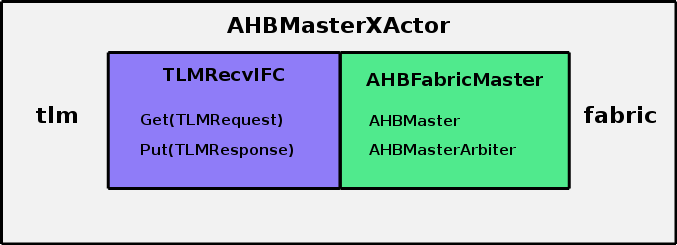
\includegraphics[height = 1 in]{AHBMasterXActor}
\caption{AHBMasterXActor Interface}
\label{AHBmasterXActor}
\end{center}
\end{figure}

\paragraph{\bf AHBMasterXActor} The \te{AHBMasterXActor} has two subinterfaces: 
an \te{AHBFabricMaster} subinterface and a \te{TLMRecvIFC}
subinterface.  The TLM interface is described in the TLM package.  The transactor converts TLM requests into the AHB
protocol, and converts the AHB response back into TLM.

% \index{AHBMasterXActor@\te{AHBMasterXActor} (interface)}        

\begin{verbatim}
interface AHBMasterXActor#(`TLM_RR_DCL, `TLM_PRM_DCL);
   interface TLMRecvIFC#(`TLM_RR)      tlm;
   (* prefix = "" *)
   interface AHBFabricMaster#(`TLM_PRM) fabric;
endinterface
\end{verbatim}

% \index{AHBSlaveXActor (transactor)}

\begin{figure}[ht]
\begin{center}
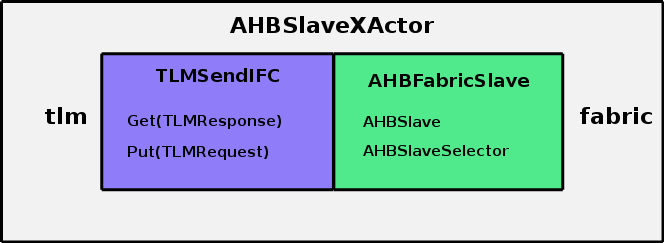
\includegraphics[height = 1 in]{AHBSlaveXActor}
\caption{AHBSlaveXActor Interface}
\label{AHBSlaveXActor}
\end{center}
\end{figure}

\paragraph{\bf AHBSlaveXActor} The \te{AHBSlaveXActor} has two subinterfaces:
\te{AHBFabricSlave} subinterface and a \te{TLMSendIFC}
subinterface. The TLM interface is described in the TLM package.
 The transactor converts an AHB request into TLM
and the TLM response back into the AHB protocol.

% \index{AHBSlaveXActor@\te{AHBSlaveXActor} (interface)}        

\begin{verbatim}
interface AHBSlaveXActor#(`TLM_RR_DCL, `TLM_PRM_DCL);
   interface TLMSendIFC#(`TLM_RR)     tlm;
   (* prefix = "" *)
   interface AHBFabricSlave#(`TLM_PRM) fabric;
endinterface
\end{verbatim}

{\bf Modules}

The following constructors are used to create AHB transactor modules.  Versions
with associated synthesis boundaries are also available. These
versions are called \te{mkAHBMasterStd}, and \te{mkAHBSlaveStd}. The specific TLM 
parameter values for these synthesized versions are as specified by the 
preprocessor macro \te{TLM\_STD\_TYPES}.

% \index{mkAHBMaster@\te{mkAHBMaster} (module)}
% \index[function]{AHB!mkAHBMaster}


\begin{center}
\begin{tabular}{|p{1.2 in}|p{5 in}|}
\hline 
&\\
\te{mkAHBMaster}&Creates an AHB Master transactor module. Provides a
\te{AHBMasterXActor} interface.  This version is polymorphic.   \\
&\\
\cline{2-2}
&\begin{libverbatim}
module mkAHBMaster (AHBMasterXActor#(`TLM_RR, `TLM_PRM))
   provisos(TLMRequestTC#(req_t, `TLM_PRM),
            TLMResponseTC#(resp_t, `TLM_PRM),
            DefaultValue#(TLMResponse#(`TLM_PRM)),
            Bits#(req_t, s0),
            Bits#(resp_t, s1),
            Bits#(RequestDescriptor#(`TLM_PRM), s2),
            AHBConvert#(AHBProt, cstm_type),
            AHBConvert#(AHBResp, cstm_type)
	    );
\end{libverbatim}
\\
\hline
\end{tabular}
\end{center}

% \index{mkAHBMasterStd@\te{mkAHBMasterStd} (module)}
% \index[function]{AHB!mkAHBMasterStd}


\begin{center}
\begin{tabular}{|p{1.2 in}|p{5 in}|}
\hline 
&\\
\te{mkAHBMasterStd}&Creates an AHB Master transactor module. Provides a
\te{AHBMasterXActor} interface.   \\
&\\
\cline{2-2}
&\begin{libverbatim}
module mkAHBMasterStd (AHBMasterXActor#(`TLM_RR_STD, `TLM_PRM_STD));
\end{libverbatim}
\\
\hline
\end{tabular}
\end{center}



% \index{mkAHBSlave@\te{mkAHBSlave} (module)}
% \index[function]{AHB!mkAHBSlave}


\begin{center}
\begin{tabular}{|p{1.2 in}|p{5 in}|}
\hline 
&\\
\te{mkAHBSlave}&Creates an AHB Slave transactor module. Provides an
\te{AHBSlaveXActor} interface.  This version is polymorphic.\\
&\\
\cline{2-2}
&\begin{libverbatim}
module mkAHBSlave#(function Bool addr_match(AHBAddr#(`TLM_PRM) addr))
                  (AHBSlaveXActor#(`TLM_RR, `TLM_PRM))
   provisos(TLMRequestTC#(req_t, `TLM_PRM),
            TLMResponseTC#(resp_t, `TLM_PRM),
            DefaultValue#(RequestDescriptor#(`TLM_PRM)),
            Bits#(req_t, s0),
            Bits#(resp_t, s1),
            AHBConvert#(AHBProt, cstm_type));
\end{libverbatim}
\\
\hline
\end{tabular}
\end{center}

% \index{mkAHBSlaveStd@\te{mkAHBSlaveStd} (module)}
% \index[function]{AHB!mkAHBSlaveStd}


\begin{center}
\begin{tabular}{|p{1.2 in}|p{5 in}|}
\hline 
&\\
\te{mkAHBSlaveStd}&Creates an AHB Slave transactor module. Provides an
\te{AHBSlaveXActor} interface.  This version is not polymorphic.\\
&\\
\cline{2-2}
&\begin{libverbatim}
module mkAHBSlaveStd#(function Bool 
                      addr_match(AHBAddr#(`TLM_PRM_STD) addr)) 
                     (AHBSlaveXActor#(`TLM_RR_STD, `TLM_PRM_STD));
\end{libverbatim}
\\
\hline
\end{tabular}
\end{center}

% \index{mkAHBSlaveDummy@\te{mkAHBSlaveDummy} (module)}
% \index[function]{AHB!mkAHBSlaveDummy}


\begin{center}
\begin{tabular}{|p{1.2 in}|p{5 in}|}
\hline 
&\\
\te{mkAHBSlaveDummy}&This is the recipient of everything that doesn't
have a slave destination. \\
&\\
\cline{2-2}
&\begin{libverbatim}
module mkAHBSlaveDummy (AHBFabricSlave#(`TLM_PRM));
\end{libverbatim}
\\
\hline
\end{tabular}
\end{center}



% \index{@\te{mkAHBBus} (module)}
% \index[function]{AHB!mkAHBBus}


The following module constructor is used to create an AHB bus fabric.

\begin{center}
\begin{tabular}{|p{1.2 in}|p{5 in}|}
\hline 
&\\
\te{mkAHBBus}&Given a vector of \te{AHBFabricMaster} interfaces and a vector 
of \te{AHBFabricSlave} interfaces, \te{mkAHBBus} creates an AHB bus fabric. \\
&\\
\cline{2-2}
&\begin{libverbatim}
module mkAHBBus#(Vector#(master_count, 
                 AHBFabricMaster#(`TLM_PRM)) masters,
		 Vector#(slv_count, AHBFabricSlave#(`TLM_PRM)) slvs) (Empty)
         provisos(Add#(slv_count, 1, slave_count));
\end{libverbatim}
\\
\hline
\end{tabular}
\end{center}



% \index{mkAHBMasterMonitor@\te{mkAHBMasterMonitor} (module)}
% \index[function]{AHB!mkAHBMasterMonitor}

The following module is used to add probe signals for each of the AHB
bus signals. This facilitates debugging and waveform viewing of the
created bus fabric.

\begin{center}
\begin{tabular}{|p{1.2 in}|p{5 in}|}
\hline 
&\\
\te{mkAHBMasterMonitor}&Adds a probe module for each of the AHB bus signals.
The \te{include\_pc} value indicates whether or not the monitor module
should include an instantiation of an AHB protocol checker module
(available from ARM).  If the protocol checker is not available, the
value of \te{include\_pc} should be set to False.  \\
&\\
\cline{2-2}
&\begin{libverbatim}
module mkAHBMasterMonitor#(AHBFabricMaster#(`TLM_PRM) master) 
                          (AHBMasterMonitor#(`TLM_PRM));
\end{libverbatim}
\\
\hline
\end{tabular}
\end{center}


% \index{getCurrentSlave@\te{getCurrentSlave} (module)}
% \index[function]{AHB!getCurrentSlave}


\begin{center}
\begin{tabular}{|p{1.2 in}|p{5 in}|}
\hline 
&\\
\te{getCurrentSlave}&  Returns the \te{slave\_num} of the current slave.\\
&\\
\cline{2-2}
&\begin{libverbatim}
module getCurrentSlave#(AHBFabricMaster#(`TLM_PRM) master, 
			Vector#(slave_count,
                        AHBFabricSlave#(`TLM_PRM)) slaves)  
                       (ReadOnly#(LBit#(slave_count)));
\end{libverbatim}
\\
\hline
\end{tabular}
\end{center}

\end{document}

% \begin{center}
% \begin{tabular}{|p{1.2 in}|p{5 in}|}
% \hline 
% &\\
% \te{}&  \\
% &\\
% \cline{2-2}
% &\begin{libverbatim}
% \end{libverbatim}
% \\
% \hline
% \end{tabular}
% \end{center}








% {\bf AHB Bridge}

% The objects described in the above sections, can be combined into a
% bridge.  This section describes design containing 2 AHB buses, bus0
% and bus1.  Each bus has a master and a slave, The master is attached
% to a randomizer, creating random data for the bus, the slave is a
% memory.  There are 2 bridges connecting the buses.  Each bridge goes
% in only one directions.

% \begin{figure}[ht]
% \begin{center}
% \includegraphics[height = 3.5 in]{AHBbridgeexample}
% \caption{AHB Bridge Example}
% \label{AHBbridge}
% \end{center}
% \end{figure}


% The \te{AHBMaster} and \te{AHBSlave} interfaces can be combined to
% form a \te{AHBBridge} interface.  This allows easy connection between
% two different AHB buses, which may have different protocols.

% The \te{AHBBridge} connects a master device, provided by the
% \te{AHBMaster} interface, to a slave device, provided by the
% \te{AHBSlave} interface.

% The \te{AHBBridge} interface has two subinterfaces; the \te{AHBMaster}
% and \te{AHBSlave}.

% \begin{libverbatim}
% interface AHBBridge#(`TLM_TYPE_PRMS);
%    interface AHBMaster master;
%    interface AHBSlave  slave;
% endinterface
% \end{libverbatim}

% % \begin{figure}[ht]
% % \begin{center}
% % \includegraphics[height = 1.2 in]{AHBbridgeinterfaces}
% % \caption{AHB Bridge Interface}
% % \label{AHBbridgeinterface}
% % \end{center}
% % \end{figure}

% The \te{AHBBridge} package provides a module to create a bridge. 


% \begin{center}
% \begin{tabular}{|p{.8 in}|p{3.8 in}|p{1.5 in}|}
%  \hline
% &  &            \\
% Module Name  &  BSV Module Declaration  & Description \\
% \hline
% \hline 
% \te{mkAHBBridge}&
% \begin{libverbatim}
% module mkAHBBridge#(function Bool addrMatch(AHBAddr a)) 
%                    (AHBBridge#(`TLM_STD_TYPES));
% \end{libverbatim}
% &Creates an AHB bridge module.\\
% \hline
% \end{tabular}
% \end{center}




